\documentclass[tikz,border=6pt]{standalone}
\usepackage{amsmath}
\usepackage{xcolor}
\usetikzlibrary{arrows.meta}

\definecolor{axisgray}{HTML}{333333}
\definecolor{lineblue}{HTML}{4A90D9}
\definecolor{linered}{HTML}{E74C3C}
\definecolor{labelgreen}{HTML}{3C763D}

\begin{document}
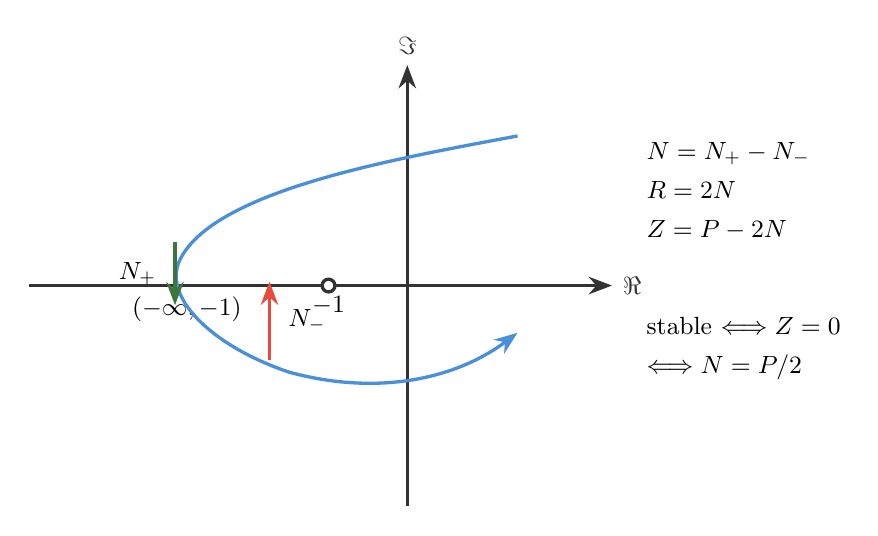
\begin{tikzpicture}[>=Stealth, line width=1.2pt, font=\small]
  \draw[axisgray, ->] (-4.8,0) -- (2.6,0) node[right] {$\Re$};
  \draw[axisgray, ->] (0,-2.8) -- (0,2.8) node[above] {$\Im$};
  \draw[axisgray, thick] (-4.6,0) -- (-1.0,0);
  \filldraw[fill=white, draw=axisgray] (-1.0,0) circle (2.3pt);
  \node[below] at (-2.8,0) {$(-\infty,-1)$};
  \node[below] at (-1.0,0) {$-1$};

  \draw[lineblue, ->] (1.4,1.9) .. controls (-0.2,1.6) and (-2.5,1.2) .. (-2.9,0.3)
    .. controls (-3.1,-0.2) and (-2.4,-0.8) .. (-1.5,-1.1)
    .. controls (-0.4,-1.4) and (0.6,-1.2) .. (1.4,-0.6);
  \draw[labelgreen, ->] (-2.95,0.55) -- (-2.95,-0.25);
  \node[left] at (-3.05,0.15) {$N_+$};
  \draw[linered, ->] (-1.75,-0.95) -- (-1.75,0.05);
  \node[right] at (-1.65,-0.45) {$N_-$};

  \node[align=left, anchor=west] at (2.9,1.2) {
    $\displaystyle N=N_+-N_-$\\[3pt]
    $\displaystyle R=2N$\\[3pt]
    $\displaystyle Z=P-2N$
  };
  \node[align=left, anchor=west] at (2.9,-0.8) {
    stable $\Longleftrightarrow Z=0$\\[3pt]
    $\Longleftrightarrow N=P/2$
  };
\end{tikzpicture}
\end{document}
